\chapter{Исследование существующих алгоритмов построения выпуклых оболочек} \label{chapt1}

\section{Существующие алгоритмы построения выпуклых оболочек} \label{sect1_1}

Построение выпуклой оболочки - это одна из первых задач, с которой зарождалась вычислительная геометрия~\cite{chadnov2004algorithmsComparison}. За долгое время развития вычислительной геометрии появилось огромное количество алгоритмов. Они работают совершенно по-разному, имеют различную сложность и скорость работы. Необходимо исследовать эти алгоритмы, чтобы использовать их лучшие черты при разработке своего. Новый алгоритм должен либо работать быстрее, либо иметь некое преимущество, которое бы являлось ключевым при выборе для использования на практике.

Все алгоритмы будут рассмотрены в предположении, что точки в изначальном множестве, поступающем на вход, находятся в общем положении. Это означает, что никакие три точки не лежат на одной прямой. Это сделано только для упрощения выкладок, на практике, конечно, необходимо рассмотреть этот случай. Он может быть учтён всеми представленными алгоритмами. Также заметим, что обычно на практике точки, лежащие на выпуклой оболочке, что невозможно при общем положении точек, не входят в состав построенной оболочки.

Для описания алгоритмов также необходимо ввести предикат $ccw(A, B, C)$, который также будет использоваться для описания алгоритмов. Предикат $ccw$ показывает точки $A, B, C$ перечислены в порядке против часовой стрелки или нет~\cite{pichardie2001formalizing}. Другими словами точка $C$ должна лежать левее прямой $A, B$. На рисунке~\ref{img:ccw_1} показано, что предикат для точек $A, B, C$ выполняется, а на рисунке~\ref{img:ccw_2} он выполняться не будет.

\begin{figure}[H]
	{\centering
		\hfill
		\subbottom[\label{img:ccw_1}]{%
			\includesvg[width=0.45\linewidth]{ccw1}}
		\hfill
		\subbottom[\label{img:ccw_2}]{%
			\includesvg[width=0.45\linewidth]{ccw2}}
		\hfill
	}
	\caption{Демонстрация работы предиката $ccw$}
	\label{img:ccw}
\end{figure}

Для того, чтобы ввести предикат $ccw$, сначала необходимо посчитать детерминант $det$, как показано в формуле~\eqref{eq:det}.

\begin{equation}\label{eq:det}
det(A, B, C)= \left| \begin{array}{ccc} x_A & y_A & 1 \\ x_B & y_B & 1 \\ x_C & y_C & 1  \end{array}\right|
\end{equation}

После чего остается только сравнить получившийся результат с нулем, что показано в формуле \eqref{eq:ccw}. Заметим, что при равенстве нулю точки будут находится на одной прямой.

\begin{equation}\label{eq:ccw}
ccw(A, B, C)=det(A, B, C) > 0
\end{equation}


\subsection{Алгоритм Джарвиса} \label{subsect1_1_1}

Алгоритм Джарвиса - это один из первых придуманных алгоритмов построения выпуклой оболочки. Он был опубликован в 1973 году \cite{jarvis1973Jarvis}. Этот алгоритм также называют алгоритмом заворачивания подарка, что отлично показывает его принцип работы.

Пусть дано множество точек $S$. Первым делом нам надо найти такую точку $t$, чтобы было известно, что она будет лежать на выпуклой оболочке. Самый простой способ сделать это - найти левую крайнюю точку. Не теряя общности рассуждений, примем найденную точку за $t_0$. Алгоритм начинает работать при $i=0$ в точке $t_0$ и выбирает такую точку $t_{i+1}$, что все остальные точки лежат правее прямой $t_i, t_{i+1}$. Также это выражается с помощью предиката \eqref{eq:ccw} в виде формулы \eqref{eq:jarvisNextPoint}.

\begin{equation}\label{eq:jarvisNextPoint}
\forall p \in S \backslash \{t_i, t_{i+1}\} : ccw(t_i, t_{i+1}, p)
\end{equation}

Прямая $t_i, t_{i+1}$ на первых шагах алгоритма показана на рисунке~\ref{img:jarvis}. Повторение этого действия пока $t_h \neq t_0$ полностью построит выпуклую оболочку изначально заданного множества. Номер последнего шага $h$ и будет количеством точек в получившейся выпуклой оболочке.

\begin{figure}[H]
    {\centering
        \hfill
        \subbottom[\label{img:jarvis_1}]{%
            \includesvg[width=0.45\linewidth]{jarvis1}}
        \hfill
        \subbottom[\label{img:jarvis_2}]{%
            \includesvg[width=0.45\linewidth]{jarvis2}}
        \hfill
    }
    \caption{Первые этапы работы алгоритма Джарвиса}
    \label{img:jarvis}
\end{figure}

Какова сложность алгоритма Джарвиса, если в множестве изначально было $n$ точек, а в выпуклую оболочку попало ровно $h$ точек? Изначальный поиск левой крайней точки занимает $n$ шагов. Поиск следующей точки $t_{i+1}$ с помощью формулы \eqref{eq:jarvisNextPoint} занимает ровно $n$ шагов. Эту операцию необходимо повторять $h$. Таким образом имеем сложность:

\[
n+ nh = O(nh)
\]

Как видно из сложности алгоритма, он зависит не только от входных данных, но и от выходных. Это интересная особенность некоторых алгоритмов построения выпуклых оболочек. В том числе от выходных данных будет зависеть и предлагаемый в данной работе алгоритм.

\subsection{Алгоритм Грэхема} \label{subsect1_1_2}

Алгоритм Грэхема - это, наверное, самый популярный из ныне используемых алгоритмов построения выпуклых оболочек. Он был опубликован в 1972 году~\cite{graham1972GrahamScan}. Алгоритм очень прост в написании и при этом работает очень эффективно.

Пусть дано множество точек $S$. Первый шаг алгоритма полностью повторяет алгоритм Джарвиса - мы находим точку с самой маленькой x-координатой. Назовём эту точку $t_0$. Теперь необходимо отсортировать все остальные точки $[t_1, t_{n-1}]$ по углу относительно точки $t_0$. Это можно сделать с помощью уже знакомого предиката ccw~\eqref{eq:ccw}. Визуально это сортировка линий $t_0, t_i$, что показано на рисунке~\ref{img:graham_sort}.

\[
A<B=ccw(t_0, A, B)
\]

\begin{figure}
	\centering
	\includesvg[width=0.6\linewidth]{graham_sort}
	\caption{Сортировка точек в алгоритме Грэхема}
	\label{img:graham_sort}
\end{figure}

Следующий этап алгоритма - это итерирование по отсортированному множеству точек. В это время все точки уже добавленные в выпуклую оболочку содержатся в стеке. Пусть сейчас добавляется точка $p$. А в стеке содержатся точки $[t_{last}, t_{last-1}, ...]$. Тогда необходимо удалить из стека такие точки, что $t_{last-1}, t_{last}, p$ образуют правый поворот. Это означает, что не выполняется $ccw(t_{last-1}, t_{last}, p)$.

На рисунке~\ref{img:graham} показан пример добавления точек при работе алгоритма Грэхема. На первом рисунке~\ref{img:graham_1} можно видеть, что добавляется точка $p_3$. Выполняется $ccw(p_1, p_2, p_3)$, поэтому точка добавляется в текущий стек. На следующем рисунке~\ref{img:graham_2} добавляется точка $p_4$, но предикат $ccw(p_2, p_3, p_4)$ не выполняется, поэтому точку $p_3$ необходимо удалить, после на рисунке~\ref{img:graham_3} видно, что это приводит к выполнению предиката $ccw(p_1, p_2, p_4)$, поэтому точка $p_4$ может быть добавлена в стек. Оставшиеся точки будут обработаны аналогичным образом, после чего мы получим готовую выпуклую оболочку состоящую из точек $p_0, p_1, p_2, p_4, p_6$.

\begin{figure}[H]
	{\centering
		\hfill
		\subbottom[\label{img:graham_1}]{%
			\includesvg[width=0.3\linewidth]{graham1}}
		\hfill
		\subbottom[\label{img:graham_2}]{%
			\includesvg[width=0.3\linewidth]{graham2}}
		\hfill
		\subbottom[\label{img:graham_3}]{%
			\includesvg[width=0.3\linewidth]{graham3}}
		\hfill
	}
	\caption{Пример добавления точек при работе алгоритма Грэхема}
	\label{img:graham}
\end{figure}

Сложность этого алгоритма очень легко проанализировать. Сначала выполняется обход множества точек в поиске самой левой точки за $O(n)$. Потом необходимо отсортировать все остальные точки за $O(n \log n)$. Потом происходит обход всех точек. Заметим, что каждая точка максимум один раз добавляется в стек и один раз удаляется из него, то есть происходит $2n$ операций, что даёт сложность $O(n)$. Итоговая сложность алгоритма равна:
\[
O(n) + O(n \log n) + O(n) = O(n \log n)
\]

\subsection{Разделяй и властвуй} \label{subsect1_1_3}

Алгоритм на основе принципа ''Разделяй и влавствуй'' был опубликован 1977 году~\cite{preparata1977DivideAndConquer}. Его разработали Препарата и Хонг.

Принцип ''Разделяй и властвуй'' является очень популярным во многих алгоритмах в информатике. Самое знаменитое его применение - это, пожалуй, сортировка слиянием. Именно от неё во многом позаимствовал этот алгоритм для построения выпуклой оболочки множества точек.

Этот алгоритм проще всего описать с помощью рекурсивной процедуры CalcHull~\cite{mount2000lecture}.

\begin{algorithm}[H]
	\caption{CalcHull - функция алгоритма Разделяй и Властвуй}
	\begin{algorithmic}[1]
		\Procedure{CalcHull}{$S$}
		\If {$|S| <= 3$}
			\Return $S$
		\EndIf
		\State $leftS\gets leftOf(S)$ \Comment{Получить левую половину множества $S$}
		\State $rightS\gets rightOf(S)$ \Comment{Получить правую половину множества $S$}
		\State $leftHull\gets CalcHull(leftS)$
		\State $rightHull\gets CalcHull(rightS)$
		\State
		\Return $mergeHulls(leftHull, rightHull)$
		\EndProcedure
	\end{algorithmic}
\end{algorithm}

Сложность данного алгоритма может быть рассмотрена с помощью рекурсии, так как это и есть рекурсивная функция. Пусть изначальное множество точек состоит из $n$ элементов. Рассмотрим всё время требующееся процедуре кроме рекурсивных вызовов. Изначально нужно разделить множество точек на $leftS$ и $rightS$. Это требует $O(n)$ времени. После чего необходимо посчитать верхнюю и нижнюю касательные, и после вывести ответ. Эти действия также занимают $O(n)$ времени, что мы покажем ниже. Таким образом время может быть описано рекурсивной формулой~\ref{eq:mergeHullAnalysisBegin}.
\begin{equation}\label{eq:mergeHullAnalysisBegin}
T(n) = 3n + 2T(n/2)
\end{equation}

Предположим, что сложность алгоритма равна $O(n \log n)$.
\[
T(n) = cn \log n
\]

По предположению индукции для всех меньших $n$ мы уже доказали, что это правда, теперь выведем для $n$.
\[
T(n) = 3n + cn \log n/2 = 3n - cn \log 2 + cn \log n = (3 - c \log 2)n + cn \log n
\]

Таким образом сложность алгоритма ''Разделяй и влавствуй'' равна:
\[
T(n) = 3/(\log 2)n \log n = O(n \log n)
\]

Единственное, что осталось доказать - это что можно вычислить верхнюю и нижнюю касательные за $O(n)$ время. Мы будем рассматривать только как считать нижнюю касательную, потому что верхняя может быть рассмотрена симметрично. Итак, пусть $a$ - это самая правая точка $leftHull$, а $b$ - это самая левая точка $rightHull$. Тогда пока $ab$ это не нижняя касательная ни для $leftHull$, ни для $rightHull$, необходимо попытаться продвинуть точку $a$ максимально вниз пока $ab$ не будет являться нижней касательной для $leftHull$, а потом продвинуть точку $b$ пока $ab$ не будет являться нижней касательной для $rightHull$. Этот процесс показан на рисунке~\ref{img:merge_1}. Финальный результат показан на втором рисунке~\ref{img:merge_2}.

\begin{figure}
	{\centering
		\hfill
		\subbottom[\label{img:merge_1}]{%
			\includesvg[width=0.45\linewidth]{merge1}}
		\hfill
		\subbottom[\label{img:merge_2}]{%
			\includesvg[width=0.45\linewidth]{merge2}}
		\hfill
	}
	\caption{Нахождение верхней и нижней касательных}
	\label{img:merge}
\end{figure}


Проверять является ли прямая нижней касательной к выпуклой оболочке очень просто. Достаточно проверить лежат ли соседние к $a, b$ точки выше этой прямой.

Очевидно, что алгоритм нахождения нижней касательной работает за $O(n)$, поэтому анализ сложности, показанный выше, верен.

\subsection{QuickHull} \label{subsect1_1_4}

Алгоритм QuickHull был создан независимо Эдди и Бикатом в 1977 и в 1979 соответственно~\cite{barber1996Quickhull}.

Как было замечено, алгоритм "Разделяй и влавствуй" во многом берёт идеи из сортировки слиянием. Логическим продолжением алгоритма, который основан на сортировке слиянием является алгоритм основанный на быстрой сортировке. Это довольно простой и в то же время быстро работающий алгоритм. В точности как и быстрая сортировка, данный алгоритм имеет сложность $O(n \log n)$. Но в худшем случае он может работать за $O(n^2)$. Что отличает алгоритм нахождения выпуклой оболочки множества точек Quickhull и алгоритм сортировки Quicksort - это невозможность случайной перестановки до работы алгоритма, чтобы алгоритм всегда работал с сложностью $O(n \log n)$.

Самая главная идея, которая лежит в основе данного алгоритма - это убирание ненужных точек, чем раньше мы их отбросим, тем лучше. Таких точек очень много внутри выпуклой оболочки. Как правило большинство точек изначального множества окажется внутри.

Первый шаг алгоритма - это найти четыре точки у которых будут минимальные/максимальные x/y-координаты. Это даёт нам изначальное приближение к выпуклой оболочке, которую мы построим в итоге. Очевидно, что точки, который будут лежать внутри получившегося четырёхугольника можно не рассматривать, так как они будут точно лежать внутри выпуклой оболочки. Это показано на рисунке~\ref{img:quickhull_first}.

\begin{figure}[H]
	\centering
	\includesvg[width=0.5\linewidth]{quickhull1}
	\caption{Первый шаг алгоритма Quickhull}
	\label{img:quickhull_first}
\end{figure}

Как видно на рисунке~\ref{img:quickhull_first} после первого шага остаются точки в четырёх угловых треугольниках описанного прямоугольника. На каждом шаге алгоритма для каждого текущего ребра выпуклой оболочки мы будем рассматривать точки, которые лежат снаружи этого ребра. Все шаги алгоритма будут заключаться в том, что мы находим самую дальнюю из всех этих точек и добавляем эту точку в выпуклую оболочку. Таким образом от каждого рассмотренного ребра добавляется ещё два новых. Этот процесс показан на рисунке~\ref{img:quickhull_second} для ребра $A, B$. Как видно на~\ref{img:quickhull_second_1} мы рассматриваем некоторое множество точек на текущем шаге и находим самую дальнюю из них $C$. После чего мы добавляем эту точку к выпуклой оболочке нашего множества, что показано на рисунке~\ref{img:quickhull_second_2}.

\begin{figure}[H]
	{\centering
		\hfill
		\subbottom[\label{img:quickhull_second_1}]{%
			\includesvg[width=0.45\linewidth]{quickhull2}}
		\hfill
		\subbottom[\label{img:quickhull_second_2}]{%
			\includesvg[width=0.45\linewidth]{quickhull3}}
		\hfill
	}
	\caption{Алгоритм Quickhull}
	\label{img:quickhull_second}
\end{figure}

Сложность алгоритма Quickhull, в точности как и quicksort, зависит от того, насколько ровно будут разбиваться точки на 2 части при добавлении самой дальней из них. Пусть $T(n)$ - это время работы алгоритма в зависимости от количества точек поступивших на вход $n$. За один проход по точкам мы можем определить точку, которая будет разбивать наше множества на 2, которые должны быть рассмотрены далее. Пусть $n_1, n_2$ - это количества точек в подмножествах после разбиения. Очевидно, что $n_1+n_2<=n$. Таким образом время может быть описано рекурсивной формулой~\ref{eq:quickHullAnalysisBegin}.

\begin{equation}\label{eq:quickHullAnalysisBegin}
T(n) = n + T(n_1) + T(n_2)
\end{equation}

Чтобы решить эту формулу, необходимо выбрать некоторые значения для $n_1$ и $n_2$. Если предположить, что точки более или менее ровно разбиваются, что описывается формулой~\ref{eq:quickHullAnalysisConstant}, то можно доказать, что время работы алгоритма будет $O(n \log n)$. Если же разбиения не ровные, то время работы алгоритма легко может стать $O(n^2)$~\cite{mount2000lecture}.

\begin{equation}\label{eq:quickHullAnalysisConstant}
\exists  a < 1 : max(n_1, n_2) <= a * n
\end{equation}

Этот алгоритм может быть очень хорош на некотором наборе точек, и чаще всего он отлично работает. Причём как видно из описания алгоритма он отбрасывает очень много ненужных точек на каждом шаге, что делает его замечательным для использования, если бы не плохое время при специально подобранном наборе точек. Поэтому на практике всё равно предпочитают алгоритм Грэхема.

\subsection{Инкрементальный алгоритм} \label{subsect1_1_5}

Инкрементальный алгоритм был опубликован Препаратом в 1979 году \cite{preparata1979Incremental}.

Инкрементальный алгоритм - это алгоритм, на который мы будем опираться больше всего при построении нашего собственного. Он использует два бинарных дерева поиска для построения выпуклой оболочки. Основная идея алгоритма в том, что мы будем добавлять точки в произвольном порядке и для текущих добавленных точек будет поддерживаться текущая выпуклая оболочка. Получается, что необходима такая структура данных, которая должна определять точка находиться внутри или снаружи выпуклой оболочки. После чего если точка находится снаружи, то необходимо её добавить к текущей выпуклой оболочке с учётом того, что необходимо удалить точки, которые уже не принадлежат выпуклой оболочке.

Эффективная структура данных для такого алгоритма - это бинарное дерево поиска. Мы будем хранить текущую выпуклую оболочку в двух деревьях. Верхнее $T_H$ и нижнее $T_L$ деревья будут представлять верхнюю и нижнюю части выпуклой оболочки. То есть, чтобы в конце получить результат необходимо слить эти две цепочки в один цикл. Эти деревья показаны на рисунке \ref{img:incremental_trees} \cite{instructor2004incremental}.

Существует 2 типа вершин, в таких деревьях:
\begin{enumerate}
	\item Внутренние вершины деревьев представляют собой пары $(v_x, v)$, где $v$ - это точка, которая сейчас находится на выпуклой оболочке, а $v_x$ - координата $x$ этой точки. Таким образом точка отсортированы по координате $x$. Они показаны кружками на рисунке \ref{img:incremental_trees}.
	\item Внешние вершины представляют собой либо ребро выпуклой оболочки, либо пустую полуплоскость в случае крайней левой и крайней правой вершин. Они показаны квадратами на рисунке \ref{img:incremental_trees}.
\end{enumerate}

\begin{figure}[ht] 
	\centering
	\includesvg[scale=0.7]{incremental1}
	\caption{Структура данных для инкрементального алгоритма}
	\label{img:incremental_trees}
\end{figure}

Опишем процесс поиска вершина снаружи или внутри в такой структуре. Пусть ищется точка $q$. Тогда необходимо в деревьях $T_H$ и $T_L$ найти ребро или вершину, которая находится в точке $q_x$. Назовём найденные точки и ребра $v_L, e_L, v_H, e_H$ для нижнего и верхнего дерева соответственно. Пример получившегося результата показан на рисунке \ref{img:incremental_locate}.

Рассмотрим 4 случая:
\begin{enumerate}
	\item Если нет таких ребёр или вершин, тогда эта точка находится снаружи выпуклой оболочки.
	\item Если точка находиться в вершине $v_L, v_H$ или на ребре $e_L, e_H$, то $q$ лежит на выпуклой оболочке.
	\item Если $q$ ниже $e_H (v_H)$ и выше $e_L (v_L)$, то $q$ лежит внутри выпуклой оболочки.
	\item Иначе $q$ лежит снаружи выпуклой оболочки.
\end{enumerate}

\begin{figure}[H] 
	\centering
	\includesvg[scale=0.7]{incremental2}
	\caption{Нахождение вершин, соответствующих точке $q$}
	\label{img:incremental_locate}
\end{figure}

Как видно, для того, чтобы определить точка лежит или снаружи необходимо сделать довольно много действий. Но как, например, определить точка $q$ находится выше ребра $a, b$  или нет? В этом снова помогает предикат $ccw$, описанный в формуле \ref{eq:ccw}. Точка находится выше если $ccw(a, b, q)$. Это показано на рисунке \ref{img:incremental_ccw}.

\begin{figure}[H]
	\centering
	\includesvg{incremental3}
	\caption{Определение положения точки с помощью предиката $ccw$}
	\label{img:incremental_ccw}
\end{figure}

После определения точка $q$ лежит внутри или снаружи выпуклой оболочки, необходимо добавить эту точку. Куда добавлять точку $q$ определяется на основе её положения. Существует 4 случая:
\begin{enumerate}
	\item Если точка лежит внутри или на выпуклой оболочке, то добавлять $q$ не нужно.
	\item Если точка снаружи сверху, то необходимо добавить её в дерево $T_H$.
	\item Если точка снаружи снизу, то необходимо добавить её в дерево $T_L$.
	\item Если точка снаружи справа или слева, то необходимо добавить её как в $T_L$, так и в $T_H$.
\end{enumerate}

Все возможные случаи показаны на рисунке \ref{img:incremental_newpoint} \cite{instructor2004incremental}.

\begin{figure}[H]
	{\centering
		\hfill
		\subbottom[Точка внутри\label{img:incremental_newpoint_1}]{%
			\includesvg[width=0.21\linewidth]{incremental4}}
		\hfill
		\subbottom[Точка снаружи сверху\label{img:incremental_newpoint_2}]{%
			\includesvg[width=0.21\linewidth]{incremental5}}
		\hfill
		\subbottom[Точка снаружи снизу\label{img:incremental_newpoint_3}]{%
			\includesvg[width=0.21\linewidth]{incremental6}}
		\hfill
		\subbottom[Точка снаружи слева\label{img:incremental_newpoint_4}]{%
			\includesvg[width=0.21\linewidth]{incremental7}}
		\hfill
	}
	\caption{Добавление новой точки в инкрементальном алгоритме}
	\label{img:incremental_newpoint}
\end{figure}


Последнее, что необходимо определить в этом алгоритме - это как правильно добавлять точку в дерево. Опишем это с помощью псевдокода \cite{incremental2005presentation} \cite{instructor2004incremental}:

\begin{algorithm}[H]
	\caption{AddPoint - функция добавления точки $q$ инкрементального алгоритма}
	\label{alg:incremental_addpoint}
	\begin{algorithmic}[1]
		\Procedure{AddPoint}{$q$}
		\State $e (v) \gets ребро (вершина), которая находится в q_x$
		\State $b \gets левый сосед e(v)$
		\State $c \gets левый сосед w$
		\While {$\neg ccw(q, b ,c)$}
			\State Удалить вершину $b$ из дерева
			\State $b \gets c$
			\State $c \gets левый сосед b$
		\EndWhile
		
		\State $b \gets правый сосед e(v)$
		\State $c \gets правый сосед w$
		\While {$\neg ccw(c, b, q)$}
			\State Удалить вершину $b$ из дерева
			\State $b \gets c$
			\State $c \gets правый сосед b$
		\EndWhile
		\State Добавить вершину $q$ в дерево
		\EndProcedure
	\end{algorithmic}
\end{algorithm}

Какова же сложность этого алгоритма? Операция поиска вершины на шаге $i$ в дереве занимает $O(\log h_i)$, где $h_i$ - это количество точек в выпуклой оболочке на шаге $i$. Функция AddPoint работает за $O((1+k) \log h_i)$, где $k$ - количество точек, которые необходимо удалить. Заметим, что для конечного множества точек $S$ каждая точка может быть добавлена и удалена только 1 раз. Что означает, что за всё время работы алгоритма будет $O(n \log h_{ср})$ операций. $h$ - это максимальная высота дерева во время работы алгоритма. В среднем случае сложность будет $O(n \log h)$, где $h$ - это количество точек в получившейся выпуклой оболочке. В худшем случае сложность равняется $O(n \log n)$ \cite{instructor2004incremental}.

Этот алгоритм используется на практике из-за своей исключительно хорошей работе на множествах, где количество точек в результирующей выпуклой оболочке получается много меньше изначального количества точек.

\subsection{Алгоритм Чана} \label{subsect1_1_6}

Алгоритм Чана - это самый лучший, с точки зрения сложности, алгоритм, существующий на сегодняшний момент. Он был опубликован в 1996 году Тимоти М. Чаном \cite{chan1996Chan}. Этот алгоритм совмещает прошлые идеи Грэхема и Джарвиса. Сложность этого алгоритма $O(n \log h)$. Нужно заметить, что это не первый алгоритм построения выпуклой оболочки, который имеет такую сложность. До этого в 1986 году был опубликован алгоритм Киркпатрика \cite{kirkpatrick1986ultimate}, который основан на методе "разделяй и властвуй", но тот алгоритм имел очень большую константу и был сложен в имплементации, поэтому его рассматривать в этой работе мы не будем.

Работа алгоритма основана на идее, что мы выполняем его для параметра $m$, который равен $h$ (количество точек в финальной выпуклой оболочке). Конечно это не так в реальной жизни, но позже мы докажем, что это не мешает постепенно увеличивать параметр $m$ и всё равно получить сложность $O(n \log h)$.

Итак рассмотрим работу алгоритма для конкретного параметра $m$. Для того, чтобы алгоритм успешно выполнился построив выпуклую оболочку необходимо выполнения условия $m >= h$.

В начале работы алгоритм разбивает изначальное множество $S$ точек на $K <= 1 + n / m$ подмножеств. В каждом из подмножеств $(Q_k)_{k=1,2,...K}$ будем по $m$ точек. Заметим, что $K = O(n / m)$.

Для каждого множества $Q_k$ из $p$ точек вычисляется выпуклая оболочка $C_k$, используя алгоритм, работающий за $O(p \log p)$, например, алгоритм Грэхема. Так как всего есть $K$ подмножеств из $O(m)$ точек, то этот шаг требует $K * O(m \log m) = O(n \log m)$ времени. Изначальное разбиение и получившиеся выпуклые оболочки показаны на рисунке \ref{img:chan_1}.

\begin{figure}[H]
	{\centering
		\hfill
		\subbottom[Разбиение на множества $(Q_k)$\label{img:chan_1_1}]{%
			\includesvg[width=0.4\linewidth]{chan_1_1}}
		\hfill
		\subbottom[Выпуклые оболочки $(С_k)$\label{img:chan_1_2}]{%
			\includesvg[width=0.4\linewidth]{chan_1_2}}
		\hfill
	}
	\caption{Первый этап алгоритма Чана для $m = 5$}
	\label{img:chan_1}
\end{figure}

Вторая фаза работает на уже построенных выпуклых оболочках $(C_k)_{k=1,2,...K}$ с помощью алгоритма Джарвиса. В начале необходимо взять некую первую точку, которая точно принадлежит выпуклой оболочке, например, самую левую точку множества $S$. Итак, на текущем шаге $i$ есть уже взятая в выпуклую оболочку точка $p_i$. Необходимо найти следующую точку $p_{i + 1} = f(p_i, S)$, такую что остальные точки из $S$ будут левее ребра $p_i, p_{i+1}$. Функция $f(p_i, S)$ зависит от предыдущей токи и множества $S$ остальных точек. Как сказано выше выпуклые оболочки $C_k$ подмножеств $Q_k$ уже известны и содержат максимум $m$ точек. Это позволяет найти следующую точку $f(p_i, Q_k)$ за $O(\log m)$ с помощью бинарного поиска.

Процесс поиска следующей точки с помощью бинарного поиска требует введения некоего порядка, при котором самой высокой точкой и будет точка $f(p_i, Q_k)$. Будем говорить, что точка $v_i$ выше точки $v_k$ относительно точки $p$, если выполняется предикат $ccw(p, v_i, v_k)$. Это показано на рисунке \ref{img:rtangent}.

\begin{figure}
	\centering
	\includesvg[width=0.6\linewidth]{rtangent_1}
	\caption{Порядок точек в выпуклой оболочке для вычисления $rtangent$}
	\label{img:rtangent}
\end{figure}

Также, ребро $e_i$ выпуклой оболочки $C$ является увеличивающим относительно $p$, если $v_{i+1}$ выше $v_i$. Иначе оно является уменьшающим\cite{geomal2012tangents}. Рассмотрим псевдокод функции $rtangent$, c помощью которой следующую точку $f(p_i, Q_k)$ можно легко найти по формуле $rtangent(p_i, C_k)$.

\begin{algorithm}
	\algnewcommand{\IIf}[1]{\State\algorithmicif\ #1\ \algorithmicthen}
	\algnewcommand{\EndIIf}{\unskip\ \algorithmicend\ \algorithmicif}

	\caption{rtangent - функция нахождения самой высокой точки относительно точки $p$ в выпуклом многоугольнике $C$}
	\label{alg:rtangent}
	\begin{algorithmic}[1]
		\Procedure{rtangent}{$p$, $C = {v_o, v_1, ..., v_{n-1}, v_n=v_0}$}
		\IIf {$v_0$ является локальным максимумом} \Return $v_0$ \EndIIf
		\State $a \gets 0, b \gets n$
		\State $A \gets$ ребро после $v_0$
		\Loop
			\State $c \gets \lfloor (a + b) / 2 \rfloor$
			\IIf {$v_c$ является локальным максимумом} \Return $v_c$	\EndIIf

			\State $C \gets$ ребро после $v_c$
			\If {$A$ увеличивающее ребро}
				\If {$C$ уменьшающее ребро}
					\State $b \gets c$
				\Else
					\If {$v_a$ выше $v_c$}
						\State $b \gets c$
					\Else
						\State $a \gets c, A \gets C$
					\EndIf
				\EndIf
			\Else
				\If {$C$ увеличивающее ребро}
					\State $a \gets c, A \gets C$
				\Else
					\If {$v_a$ ниже $v_c$}
						\State $b \gets c$
					\Else
						\State $a \gets c, A \gets C$
					\EndIf
				\EndIf
			\EndIf
			
			\If {$b \leq a+1$}
				\Return error - слишком маленькая цепь
			\EndIf
		\EndLoop
		\EndProcedure
	\end{algorithmic}
\end{algorithm}

Таким образом можно найти $f(p_i, Q_k)$ для всех $k=1,2,...K$. После чего используя обычный алгоритм Джарвиса необходимо линейным поиском найти среди этих точек подходящую нам $p_{i+1}$. Сложность этих шагов будет равна $O(K \log m) + O(K) = O(K \log m)$. Это необходимо делать для $h$ шагов, так как всего $h$ точек необходимо найти. В итоге сложность будет равна $O(K h \log m) = O(n \log h)$, если $m$ примерное равен $h$.

С помощью алгоритма описанного выше можно найти выпуклую оболочку множества точек $S$ из $n$ точек за $O(n \log h)$ времени. Получившийся результат пунктиром показан на рисунке \ref{img:chan_2}. Как видно некоторые рёбра получившейся выпуклой оболочки проходят по ребрам оболочек $C_k$, а некоторые их соединяют.

\begin{figure}
	\centering
	\includesvg[width=0.6\linewidth]{chan_2}
	\caption{Результат работы алгоритма Чана}
	\label{img:chan_2}
\end{figure}

Если $m$ было выбрано неправильно, то после $m$ шагов во второй фазе алгоритм будет прерван. Заметим, что в этом случае будет потрачено $O(n \log m)$ без результата. Очевидно, что необходимо подбирать число $m$ постепенно его увеличивая. Но насколько быстро увеличивать $m$? Если $m$ будет перебираться с маленьким шагом, то будет слишком много итераций алгоритма, и, очевидно, в этом случае сложность алгоритма будет много больше $O(n \log h)$. Если же шаг будет слишком большой, то сложность скатиться в $O(n \log n)$.

Одной из возможных стратегий выбора $m$ может быть увеличение возведением в квадрат. Начиная с значения $2$, $m$ на итерации $i$ выбирается по закону:
\[
m = \min (n,2^{2^t})
\]

Алгоритм заканичает работу, когда $m = 2^{2^t} >= h$. Из этого следует:
\[
m = 2^{2^t} \geq h \iff \log 2^{2^t} \geq \log h \iff 2^t \geq \log h \iff \iff t \geq \log \log h
\]

Таким образом общее время работы алгоритма:
\[
\sum_{i=1}^{\lceil \log \log h \rceil} O(n \log 2^{2^t}) = O(n) \sum_{i=1}^{\lceil \log \log h \rceil} O(2^t) = O(n 2^{1+\lceil \log \log h \rceil}) = O(n \log h)
\]

\section{Применение выпуклой оболочки при вычислении дескрипторов объектов на изображении}

\subsection{Определение дескриптора}

Итак, зачем можно применять построение выпуклой оболочки в компьютерном зрении? Ответ прост. Главное применение выпуклых оболочек состоит в описании формы объекта. Заметим, что существует множество параметров, которые могут описывать форму объекта.

Для того, чтобы понять, как применяются выпуклые оболочки при вычисления дескрипторов объектов на изображении, необходимо понять зачем он нужен и каким свойствам должен удовлетворять.

Что же такое дескриптор? Дескриптор - это конечное множество чисел, которые описывают некоторую форму или другие характеристики объекта, такие как цвет или текстура. При этом дескриптор не гарантирует однозначное восстановление формы из него. Главное, чтобы сильно различные объекты давали сильно различимые дескрипторы, а слабо различимые - похожие дескрипторы \cite{morse2000lecture}.

Объекты совершенно разной формы должны давать совершенно разные дескрипторы, когда же объекты похожей формы должны давать похожие дескрипторы. Но как понять насколько объекты различны? На этот ответ нет чёткого ответа. Люди придумывают всё больше и больше возможностей описывать формы. Некоторые лучше различают объекты, некоторые хуже, но никакой количественной оценки нет. Есть только эффективность работы дескриптора объекта на практике.

Также заметим, что желательно, чтобы значение дескриптора независело от масштаба сдвига и других афинных преобразований объекта\cite{azadeh2013lecture}. Это свойство показано на рисунке \ref{img:descriptor_invariant}.

\begin{figure}[H]
	\centering
	\includesvg[width=\linewidth]{descriptor_invariant}
	\caption{Инвариант дескриптора при масштабе и повороте}
	\label{img:descriptor_invariant}
\end{figure}

Пример того, зачем нужно это свойство, показан на рисунке \ref{img:photos}. Как мы видим на этих фотографиях один и тот же памятник был сфотографирован с разных ракурсов. Наша цель в том, чтобы сопоставить фотографии друг с другом и понять, что на них находиться один и тот же объект.

\begin{figure}[H]
	{\centering
		\hfill
		\subbottom[\label{img:photo_near}]{%
			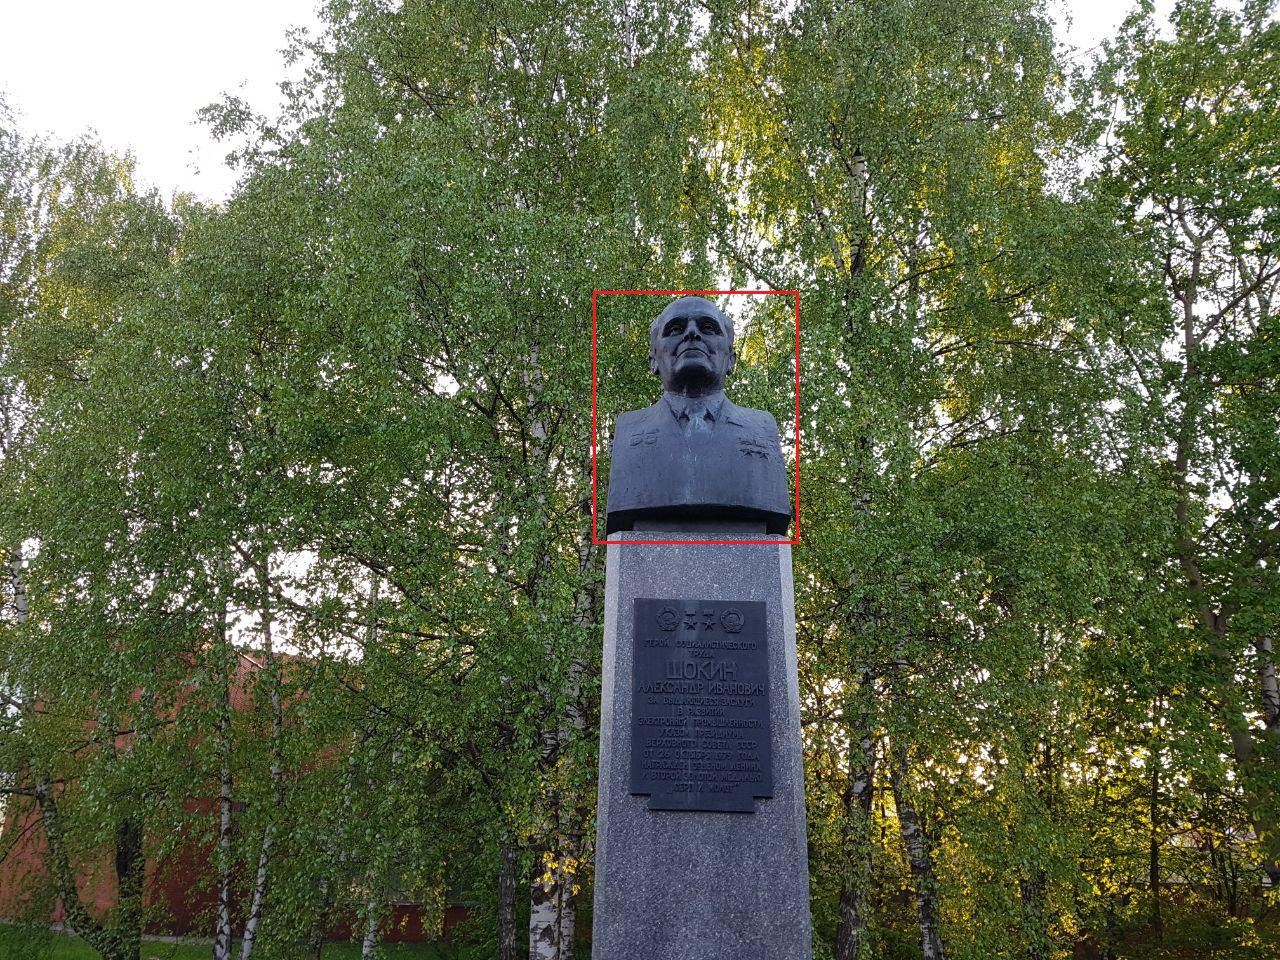
\includegraphics[width=0.49\linewidth]{photo_near}}
		\hfill
		\subbottom[\label{img:photo_far}]{%
			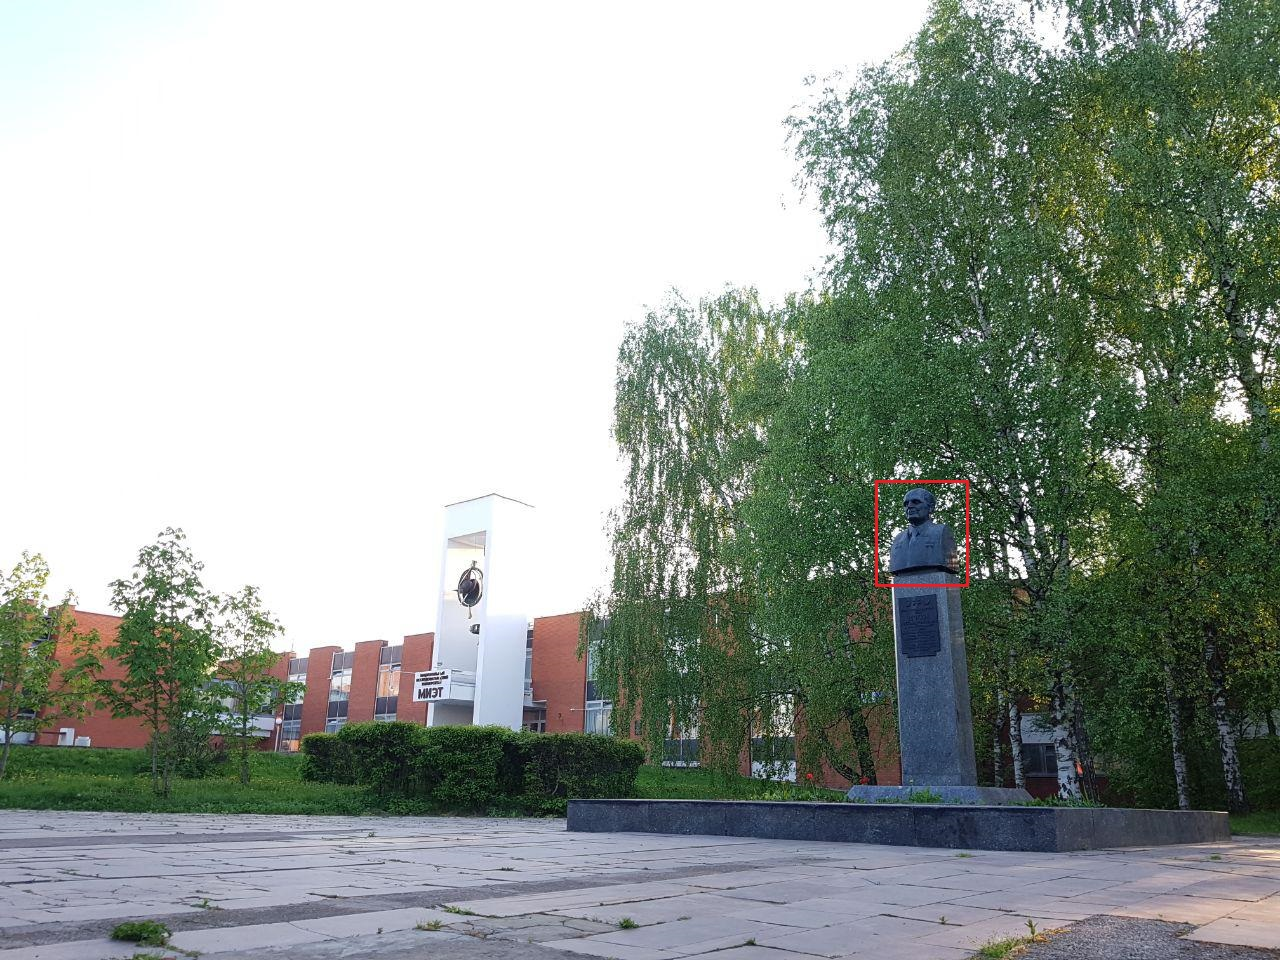
\includegraphics[width=0.49\linewidth]{photo_far}}
		\hfill
	}
	\caption{Пример объекта, сфотографированного с разных ракурсов}
	\label{img:photos}
\end{figure}

\subsection{Базовые примеры дескрипторов}

Одни из самых простых дескрипторов это:
\begin{itemize}
	\item площадь;
	\item периметр;
	\item эксцентриситет;
	\item удлинение;
	\item квадратность;
	\item ориентация \cite{morse2000lecture}.
\end{itemize}

И это лишь самые простые из возможных числовых параметров некоторой формы. Заметим, что не все из предложенных характеристик удовлетворяют устойчивости к изменению масштаба, например. Площадь как количество пикселей явно не сможет нормально описать объект. Чтобы обойти это ограничение создатели дескрипторов часто приводят описываемые объекты к одному масштабу.

Построение выпуклой оболочки необходимо скорее для дескрипторов прямо основанных на ней \cite{mathew2015content} или для дескрипторов, описывающих границы объекта, так как границой может быть и выпуклая оболочка.

\subsection{Фурье дескрипторы}

Одним из самых популярных дескрипторов объектов на изображении являются Фурье дескрипторы. Нам они особенно интересны, потому что описывают границу объекта.

Так как мы имеем дело с изображением, то можно каждый пиксель представляет из себя пару координат $(x, y)$. Это даёт возможность рассматривать точки на изображении как комплексные числа $f(k) = x(k) + iy(k), k = 0,1,...,N-1$ \cite{kolyuchkin2013visionAlgorithms}. Таким образом, $x$ - это действительная часть, а $y$ - это мнимая часть комплексного числа.

По сути мы свели двумерную задачу к одномерной, что даёт нам использовать дискретное преобразование Фурье \eqref{eq:fourierDiscrete} для массива $f(k)$.

\begin{equation}\label{eq:fourierDiscrete}
F(u) = 1/N \sum_{k=0}^{N-1} f(k) \exp(- 2\pi u k / N), u = 0,1,...,N-1
\end{equation}

Комплексные коэффициенты $F(u)$ называются фурье-дескрипторами границы. Вектор признаков формируется $F(u)$ с положительными и отрицательными индексами $u = \pm 1 ,\pm 2, ..., \pm L/2$ причём $L \leq N-1$ \cite{kolyuchkin2013visionAlgorithms}.

Что насчёт инвариантности этого дескриптора? К сожалению этот дескриптор в таком виде хоть и простой, но зависим как от масштаба, так и от перемещения. Чтобы комплексные числа были независимы от перемещения, $f(k)$ считаются с учётом некоего центра $g=(x_g,y_g)$ объекта, чаще всего это центр тяжести точек \eqref{eq:descriptorCenter} \cite{thang2010fourier}.

\begin{equation}\label{eq:descriptorCenter}
f(k)=(x(k)-x_g)+i(y(k)-y_g)
\end{equation}

Инвариантность относительно масштаба объекта достигается с помощью нормировки дескрипторов на модуль дескриптора с индексом $u=1$. Тогда вектор признаков примет вид \cite{kolyuchkin2013visionAlgorithms}:

\[
X=\left(\frac{\lvert{F_{-L/2}}\rvert}{\lvert{F_1}\rvert},...,\frac{\lvert{F_{-2}}\rvert}{\lvert{F_1}\rvert},\frac{\lvert{F_2}\rvert}{\lvert{F_1}\rvert},...,\frac{\lvert{F_{L/2}}\rvert}{\lvert{F_1}\rvert}\right)^T
\]

Значение параметра $L$ определяет размерность признакового пространства $K=L-2$ \cite{kolyuchkin2013visionAlgorithms}.

\subsection{Применение выпуклой оболочки}

Очевидно, что и выпуклая оболочка может помочь описать форму объекта. Достаточно лишь посчитать выпуклую оболочку и потом каким-то образом её охарактеризовать. Исследователи уже давно используют выпуклые оболочки для того, чтобы считать дескрипторы объектов на изображении \cite{dalitz2013fourier, mathew2015content}.

Даже обычные алгоритмы расчёта дескрипторов (которые основаны на границе объекта) могут быть использованы для описания выпуклой оболочки. Более того, то, где находятся точки на выпуклой оболочке показывает форму объекта, что показано на рисунке \ref{img:alpha_convex_hull}. Как видно в некоторых местах точек больше, в некоторых меньше, это показывает, что слева снизу объект является выпуклым, когда же слева сверху, он вогнутый.

\begin{figure}[H]
	\centering
	\includesvg[scale=0.5]{alpha_convex_hull}
	\caption{Точки выпуклой оболочки символа альфа}
	\label{img:alpha_convex_hull}
\end{figure}

\section{Анализ текущего состояния алгоритмов и выявление проблемы} \label{sect1_2}

Как было сказано, выпуклые оболочки могут легко использоваться для того, чтобы описывать объекты на изображении. И надо заметить, что очень часто вычисления происходят в реальном времени, например, обработка видео-потока с камеры. Для того, чтобы быстро вычислять дескрипторы, нужны быстрые алгоритмы. Причём они должны использоваться в каждой части вычисления.

Эта работа прежде всего сконцентрирована на оптимизации части вычисления выпуклой оболочки объекта.

Почему же нас не устраивают все те алгоритмы, которые давно уже были придуманы? Есть несколько причин. Рассмотрим самый быстрый, судя по сложности алгоритма, алгоритм Чана. Алгоритм Чана хоть и является оптимальным по сложности, всё же уступает другим алгоритмам в константе, которая скрывается за этой сложностью. У алгоритма множество этапов, и он явно проигрывает по времени работы остальным алгоритмам. На это явно указывает его отстутвие во всех популярных библиотеках для компьютерного зрения: OpenCV\cite{opencvconvexhull}, CGAL\cite{cgalconvexhull} и другие.

Но какой алгоритм тогда используется? Используется алгоритм Грэхема и другие алгоритмы за $O(n \log n)$. Хоть он и не является оптимальным он самый быстрый, потому что сортировка (самый долгий этап алгоритма) уже давно оптимизирована и написана настолько хорошо, что константа становится очень маленькой.

Именно в этом и заключается проблема. С одной стороны есть оптимальный с точки зрения сложности алгоритм, который не используется, а с другой алгоритм, не являющийся оптимальным, но активно применяющийся на практике.

Ассимтотика числа вершин выпуклой оболочки для $n$ точек явно показывает, что преобладает малое количество точек в итоговой выпуклой оболочке. При равномерном распределении внутри круга - $\theta(n^{1/3})$; при равномерном распределении внутри фиксированного выпуклого многоугольника - $\theta(\log n)$; при двумерном нормальном распределении - $\theta((\log n)^{1/2})$ \cite{algolist2010convexhull}.

Получается, что для малого набора точек в итоговой выпуклой оболочке мы имеем время работы, которое явно можно улучшить.

\section{Выводы} \label{subsect1_4}

В итоге анализа текущего состояния проблемы можно с уверенностью сказать, что необходимо пересмотреть этап построения выпуклой оболочки и сделать его более эффективным.

Неоходимо разработать алгоритм, который хорошо бы работал на множествах точек, малое количество из которых на самом деле будет в выпуклой оболочке. Это прежде всего означает, что алгоритм должен иметь сложность $O(n \log h)$ в среднем случае.

Также необходимо не забывать о применении этого алгоритма, он будет применятся в первую очередь для построения выпуклых оболочек с последующим вычислением дескриптора, и если можно получить некую дополнительную информацию об объекте, то это отличит наш алгоритм в лучшую сторону по сравнению с самым популярным алгоритмом Грэхема.

